\section{Auswertung}
\label{sec:Auswertung}
Mittelwert der Federkonstanten $\symup{D} = \frac{\symup{F}}{\symup{\triangle x}}$ für $n = 10$ Messdaten ist 
\begin{equation}
\langle \symup{D} \rangle = \frac{1}{n} \sum_{i=1}^n \symup{D_i} = \SI{0.029}{\newton\per\centi\meter}.
\end{equation}
Für diese Rechnung wurde kein Programm, lediglich ein Taschenrechner verwendet.
  
Die lineare Ausgleichsrechnung ist ersichtlich aus folgender \autoref{fig:plot}.

\begin{figure}
  \centering
  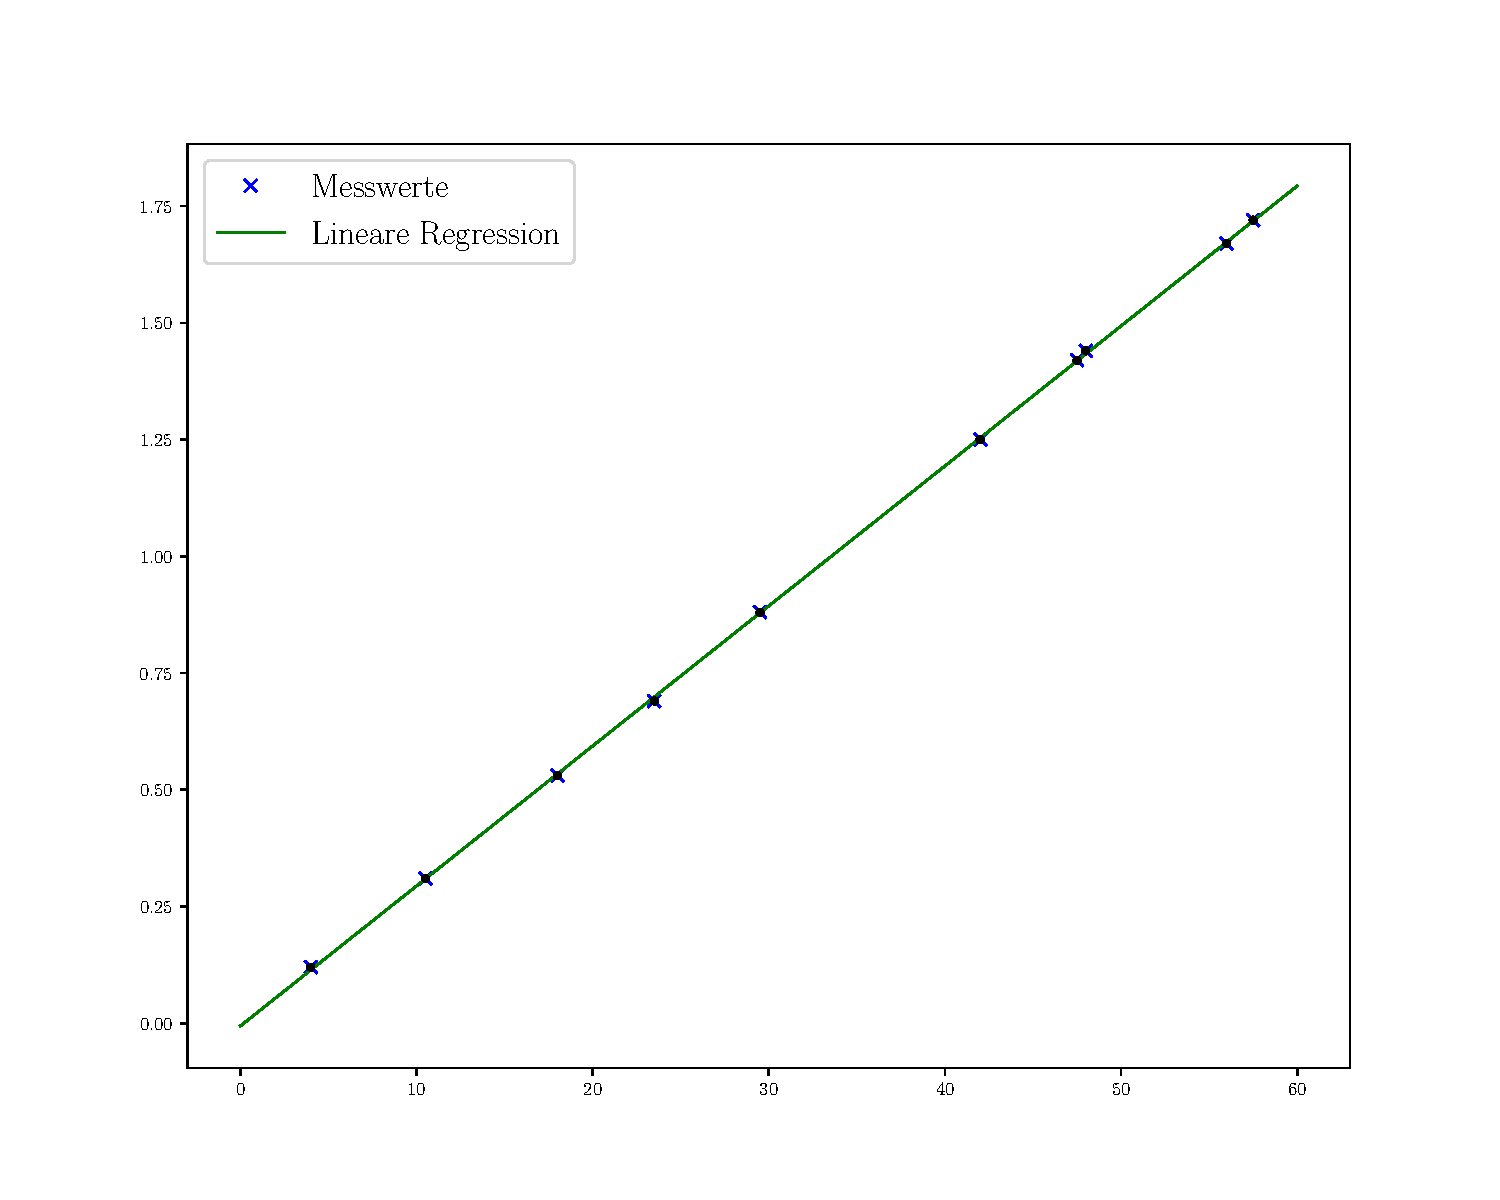
\includegraphics[max width=\linewidth]{Plot.pdf}
  \caption{Plot.}
  \label{fig:plot}
\end{figure}